\section{Odziv sustava s više stupnjeva slobode na pobudu sinusnom
silom}\label{mdof_prisilne}
Kao što je pokazano u poglavlju \ref{slobodne_oscilacije}, jednadžba gibanja sustava
s $N$ stupnjeva slobode zadana je kao sustav od $N$ diferencijalnih jednadži drugog
reda. U slučaju pobude harmonijskom silom, navedeni sustav će se sastojati od $N$
nehomogenih diferencijalnih jednadžbi drugog reda, koje će biti povezane preko
matrice krutosti i/ili matrice mase. 
\par
Općenito, rješenje jedne proizvoljne nehomogene diferencijalne jednadžbe drugog reda
oblika $\alpha\ddot{y}+\beta\dot{y}+\gamma y= f(t)$ jest suma komplementarnog
rješenja $y_c$ i partikularnog rješenja $Y_p$, pri čemu su $\alpha$, $\beta$ i
$\gamma$ konstantni koeficijenti.
\begin{equation}
    y(t)=y_c(t)+U_p(t)
\end{equation}

Komplementarno rješenje dobijemo izjednačavanjem diferencijalne jednadžbe s nulom
odnosno:
\begin{equation}\label{eq:opce_komplementarno_rjesenje}
    \alpha\ddot{y}+\beta\dot{y}+\gamma y=0
\end{equation}

Primjetimo da je komplementarno rješenje (rješenje jednadžbe \eqref{eq:opce_komplementarno_rjesenje}) 
zapravo rješenje homogene diferencijalne jednadžbe, a jednako je i za slobodne 
oscilacije i za prisilne oscilacije. Kod prisilnih oscilacija, komplementarno 
rješenje predstavlja \textit{prolazni} dio odziva te je dato u \eqref{eq:opce_rjesenje_sustava}. 
Potrebno je još odrediti partikularno rješenje, koje kod prisilnih oscilacija
predstavlja \textit{prisilni} dio odziva. Partikularno rješenje moguće je pronaći
koristeći se metodom neodređenih koeficijenata. 
\par

Zadana je jednadžba gibanja sustava s dva stupnja slobode prikazanog na slici
\ref{fig:nepriguseni_sustav-2dof}

\begin{equation}\label{eq:jednadzba_gibanja_matricno}
    \begin{bmatrix}
        m_1 & 0 \\
        0   & m_2
    \end{bmatrix}
    \begin{Bmatrix}
        \ddot{u}_1\\
        \ddot{u}_2
    \end{Bmatrix}
    +
    \begin{bmatrix}
        k_1+k_2 & -k_2\\
        -k_2 & k_2
    \end{bmatrix}
    \begin{Bmatrix}
        u_1\\
        u_2
    \end{Bmatrix}
    =
    \begin{Bmatrix}
        p_0\\
        0 
    \end{Bmatrix}
    \sin(\omega t)
\end{equation}

Odnosno:
\begin{equation}\label{eq:jednadzba_gibanja_matricno_kratko}
    \mm\vtor{u}{:}+k\vtor{u}{}=\vtor{p_n}{}\sin(\omega t)
\end{equation}

Gdje je $\vtor{p_n}{}$ vektor amplituda harmonijskih sila. Odziv sustava biti će
harmonijski, jednake frekvencije, pa partikularno rješenje možemo pretpostaviti:
\begin{equation}\label{eq:partikularno_pretpostavka}
    \vtor{u_p(t)}{}=\vtor{U_n}{}\sin(\omega t)
\end{equation}
Gdje je $\vtor{U_n}{}$ vektor koeficijenata.
Druga derivacija \eqref{eq:partikularno_pretpostavka} glasi:
\begin{equation}\label{eq:partikularno_pretpostavka_dd}
    \{\ddot{u}(t)\}=-\omega^2\vtor{U_n}{}\sin(\omega t)
\end{equation}

Uvrštavanjem \eqref{eq:partikularno_pretpostavka} i \eqref{eq:partikularno_pretpostavka_dd}
u \eqref{eq:jednadzba_gibanja_matricno_kratko} dobijemo:
\begin{equation}\label{eq:neodredjeni_koeficijenti_1}
    -\omega^2\vtor{U_n}{}\mm\sin(\omega t) 
    +
    \vtor{U_n}{}\kk\sin(\omega t)
    =
    \vtor{p}{}\sin(\omega t)
\end{equation}

Nakon sređivanja, jednadžba \eqref{eq:neodredjeni_koeficijenti_1} poprima oblik:
\begin{equation}\label{eq:neodredjeni_koeficijenti_2}
    [\kk-\omega^2\mm]\vtor{U_n}{}=\vtor{p}{}
\end{equation}

%Matrica $[\kk-\omega^2\mm]$ predstavlja matricu dinamičke krutosti sustava s više stupnjeva
%slobode, a označava se kao $[Z(\omega)]$. Jednadžbu pod \eqref{eq:neodredjeni_koeficijenti_2}
%možemo zapisati kao:
%\begin{equation}\label{eq:neodredjeni_koeficijenti_z}
%    [Z(\omega)]\vtor{U_n}{}=\vtor{p_n}{}
%\end{equation}
%
%Konačno, vektor koeficijenata dobijemo množenjem izraza \eqref{eq:neodredjeni_koeficijenti_z}
%inversom matrice dinamičke krutosti, te dobijemo:
%\begin{equation}
%    \vtor{U_n}{}=\vtor{p_n}{}\,[Z(\omega)]^{-1}
%\end{equation}

Množenjem jednadžbe \eqref{eq:neodredjeni_koeficijenti_2} s $[\kk-\omega^2\mm]^{-1}$
dobijemo:
\begin{equation}
    \begin{split}
        \vtor{U_n}{}=[\kk-\omega^2\mm]^{-1}\vtor{p_n}{} \notag\\
        \vtor{U_n}{}=\frac{1}{det[\kk-\omega^2\mm]}adj[\kk-\omega^2\mm]\vtor{p_n}{}\label{eqneodredjeni_koeficijenti_3}
    \end{split}
\end{equation}

Odnosno u matričnom obliku:
\begin{equation}
    \begin{Bmatrix}
        U_1\\
        U_2
    \end{Bmatrix}
    =
    \frac{1}{det[\kk-\omega^2\mm]}
        \begin{bmatrix}
            k_2-m_2\omega^2 & k_2\\
            k_2 & k_1+k_2-m_1\omega^2
        \end{bmatrix}
        \begin{Bmatrix}
            p_0\\
            0
        \end{Bmatrix}
\end{equation}

Komponente vektora $\vtor{U_n}{}$ glase:
\begin{align}
    U_1=\frac{p_0(k_2-m_2\omega^2)}{m_1m_2(\omega^2-\omega_1^2)(\omega^2-\omega_2^2)} \label{eq:vtor_1_opce}\\
    U_2=\frac{p_0k_2}{m_1m_2(\omega^2-\omega_1^2)(\omega^2-\omega_2^2)}\label{eq:vtor_2_opce}
\end{align}

Za $m_1=2m$, $m_2=m$, $k_1=2k$ i $k_2=k$ vektori glase:
\begin{align}
    U_1=\frac{p_0(k-m\omega^2)}{2m^2(\omega^2-\omega_1^2)(\omega^2-\omega_2^2)}\label{eq:vtor_1}\\
    U_2=\frac{p_0k}{2m^2(\omega^2-\omega_1^2)(\omega^2-\omega_2^2)}\label{eq:vtor_2}
\end{align}

Uz $\omega_1=\sqrt{k/2m}$ i $\omega_2=\sqrt{2k/m}$ te dijeljenjem \eqref{eq:vtor_1} i \eqref{eq:vtor_2}
s $p_0/2k$ dobijemo vektor dinamičkog koeficijenta pomaka (bez dimenzija), koji ovisi o
omjerima frekvencija $\omega/\omega_1$ te $\omega/\omega_2$. Vektor je prikazan u nastavku
\begin{equation}
    \frac{2k}{p_0}\vtor{U}{}
    =
    \begin{Bmatrix}
        \ffrac{1-0.5(\omega/\omega_1)^2}
              {[1-(\omega/\omega_1)^2][1-(\omega/\omega_2)^2]}\\[12pt]
        \ffrac{1}
              {[1-(\omega/\omega_1)^2][1-(\omega/\omega_2)^2]}
    \end{Bmatrix}
\end{equation}

Prisilni dio odziva glasi:
\begin{equation}
    \vtor{u(t)}{} = \frac{2k}{p_0}\vtor{U}{}\sin(\omega t) = 
    \begin{Bmatrix}
        \ffrac{1-0.5(\omega/\omega_1)^2}
              {[1-(\omega/\omega_1)^2][1-(\omega/\omega_2)^2]}\\[12pt]
        \ffrac{1}
              {[1-(\omega/\omega_1)^2][1-(\omega/\omega_2)^2]}
    \end{Bmatrix}
    \sin(\omega t)
\end{equation}

Komponente vektora $\vtor{U}{}$ možemo iscrtati kao graf funkcije dinamičkog faktora
$U_1/p_0/2k$ i $U_2/p_0/2k$ u ovisnosti o frekvencijskom omjeru $\omega/\omega_1$.
\begin{figure}[H]
    \begin{subfigure}[t]{1\textwidth}
        \centering
        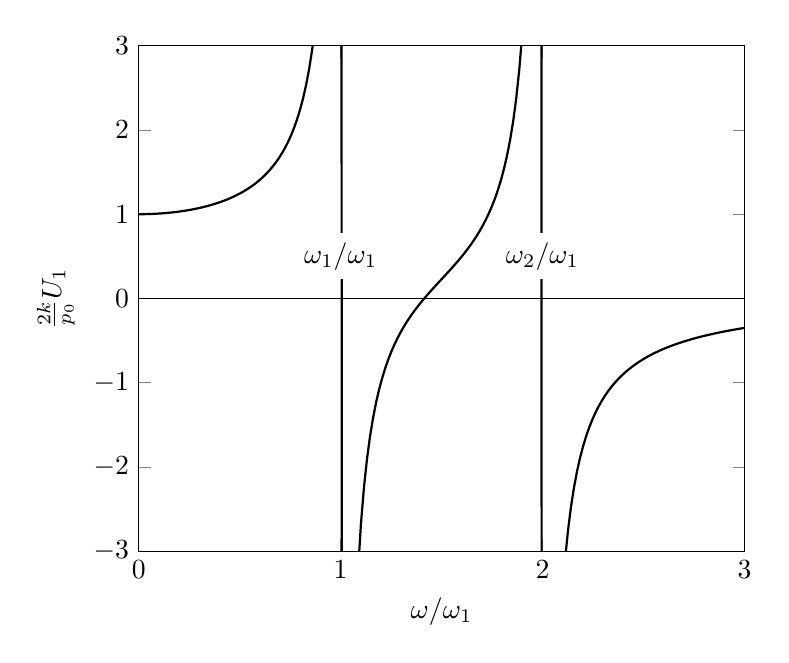
\begin{tikzpicture}
    \begin{axis} [
        height=8cm,
        ylabel = $\frac{2k}{p_0} U_1$,
        xlabel = $\omega/\omega_1$,
        xmin = 0, xmax = 3,
        ymin = -3, ymax = 3,
        xtick = {0, 1, 2, 3},
        ytick = {-3, -2, -1, 0, 1, 2, 3},
     ]
        \addplot [
            domain=0:3,
            samples=200,
            color=black,
            thick,
        ]{(1 - 0.5 * x^2)/((1-x^2) * (1-0.25 * x^2))};

        \node[rectangle,fill=white] at (1, 0.5) {$\omega_1/\omega_1$};
        \node[rectangle,fill=white] at (2, 0.5) {$\omega_2/\omega_1$};
        \draw[thin] (0, 0) -- (3, 0);
    \end{axis}
\end{tikzpicture}



    \end{subfigure}
    \vfill
    \begin{subfigure}[b]{1\textwidth}
        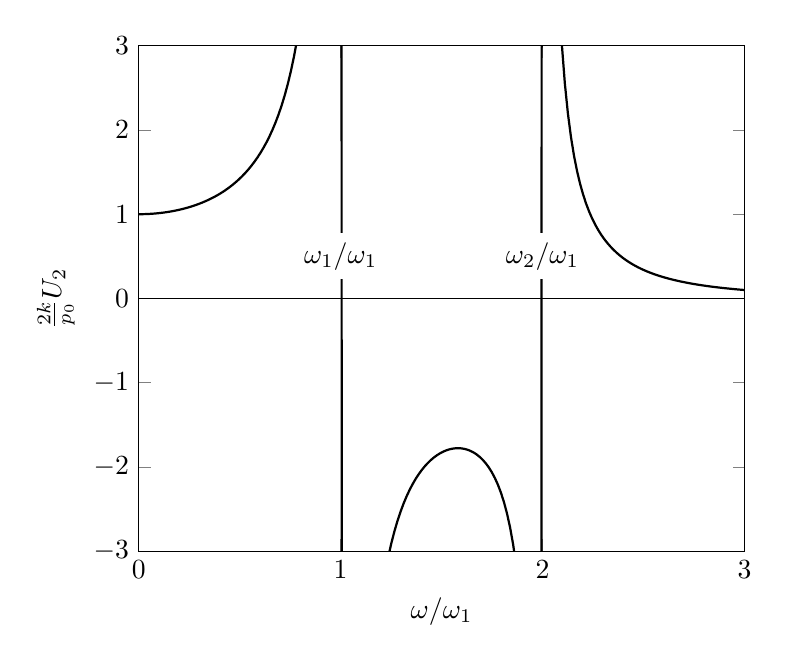
\begin{tikzpicture}
    \begin{axis} [
        height=8cm,
        ylabel = $\frac{2k}{p_0} U_2$,
        xlabel = $\omega/\omega_1$,
        xmin = 0, xmax = 3,
        ymin = -3, ymax = 3,
        xtick = {0, 1, 2, 3},
        ytick = {-3, -2, -1, 0, 1, 2, 3},
    ]
        \addplot [
            domain=0:3,
            samples=200,
            color=black,
            thick,
        ]{1/((1-x^2) * (1-0.25 * x^2))};

        \node[rectangle,fill=white] at (1, 0.5) {$\omega_1/\omega_1$};
        \node[rectangle,fill=white] at (2, 0.5) {$\omega_2/\omega_1$};
        \draw[thin] (0, 0) -- (3, 0);
    \end{axis}
\end{tikzpicture}


    \end{subfigure}
    \caption{Grafički prikaz vektora $U$ po komponentama $U_1$ i $U_2$}
    \label{fig:vektor_dinamicki_faktor}
\end{figure}

Grafovi sa slike \ref{fig:vektor_dinamicki_faktor} ukazuju na postojanje dviju
rezonancijskih frekvencija: $\omega_1$ i $\omega_2$, pri čemu je dinamički faktor
neomeđen.
